\documentclass[12pt]{article}

\usepackage{fullpage}
\usepackage{graphicx, rotating, booktabs} 
\usepackage{times} 
\usepackage{natbib} 
\usepackage{indentfirst} 
\usepackage{setspace}
\usepackage{grffile} 
\usepackage{hyperref}
\usepackage{adjustbox}
\usepackage{amsmath}
\setcitestyle{aysep{}}


\singlespace
\title{\textbf{Alliance Participation and Military Spending}}
\author{Joshua Alley\footnote{Graduate Student,
Department of Political Science, Texas A\&M University.}}
\date{{\normalsize \today}}

\bibliographystyle{apsr}

\begin{document}

\maketitle 

\doublespace 

\begin{abstract}
How does alliance participation change military spending? 
Some have argued that joining an alliance leads to greater defense expenditures, while others contend that alliances lead to spending cuts.
I argue both views are correct under certain conditions; alliance participation can raise or lower growth in military expenditures, depending on treaty scope and state capability. 
Major powers, the most capable states, use alliances and military spending to increase their influence in international relations, so joining an alliance usually raises their military spending. 
Less capable non-major powers focus on security from alliances and military spending, so alliance participation typically lowers their military spending. 
Issue linkages in broad alliance treaties increase major power influence and decrease non-major power freedom to lower defense spending. 
As a result, increasing treaty scope reduces the impact of alliance participation on major power military spending, but increases it for non-major powers. 
I test the argument by creating a measure of alliance treaty scope and employing that measure in a multilevel model. 
The research design generates new empirical evidence linking alliance participation and growth in state military spending from 1816 to 2007. 
I find that greater treaty scope increases growth in military spending in non-major powers and decreases spending growth for major powers.  
These results help scholars and policymakers better understand a central question about alliance politics that has been debated in scholarship for decades. 
\end{abstract}


\newpage 


\section{Introduction}


Scholars of international relations have long acknowledged that there are two ways for states to increase their security. 
States can invest in indigenous military capability or form alliances \citep{Morgenthau1948, Altfield1984, Morrow1993}.
Because both policies provide security, broadly defined, alliance participation should change how states invest in military capability. 
But exactly how alliances influence military spending remains unclear. 


Existing scholarship produces competing predictions and evidence on the question of alliance participation and military spending. 
One view, which I call the \textit{force multiplier perspective} expects alliance participation will reduce military spending \citep{Morrow1993, Conybeare1994, DigiuseppePoast2016}. 
The other view, which I label the \textit{foreign entanglement perspective}, predicts alliance participants will spend more on defense \citep{Diehl1994, MorganPalmer2006}. 
This paper addresses the theoretical and empirical division by clarifying when alliance participation leads to more or less defense spending. 
In doing so, it helps clarify a longstanding debate about alliance politics.


Debate between the force multiplier and foreign entanglement perspectives largely ignores heterogeneity among alliances, which is essential to alliance politics scholarship \citep{Morrow1991, Leeds2003, LeedsAnac2005, Fordham2010, Mattes2012, Benson2012, Poast2013, Johnsonetal2015}.  
Alliance participation could plausibly increase or decrease defense expenditures. 
I use state capability and treaty scope to explain when alliance treaty participation increases or decreases military spending. 


Treaties with broad scope add depth to promised military support by committing to additional cooperation.
Broad alliances cover multiple issues beyond core commitments of military intervention, including extra defense cooperation, forming international organizations, or improving economic ties.  
Changing treaty scope alters the consequences of alliance participation. 
How treaty scope modifies the impact of alliance participation on military expenditures depends on state capability because major and non-major power states use alliances and military spending for different purposes. 


Major powers use a mix of alliances and military spending to increase their influence--- shaping international relations to match their interests.
Because major powers support their alliances to gain influence, alliance participation usually increases their growth in military spending. 
Through issue-linkages, broad treaties give more influence than narrow treaties.
Thus, participation in broad treaty commitments generates lower growth in major power military spending than participation in a narrow treaties.  


Non-major powers use alliances and defense expenditures to ensure their territorial security.
Because alliances provide extra security, alliance participation often reduces non-major power growth in military spending.   
Increasing treaty scope constrains non-major powers tendency to reduce defense spending in alliances, however. 
Adding cooperation on other issues makes an alliance more valuable and gives partners greater influence through issue linkages. 
Thus, participation in broad treaties increases growth in non-major power military expenditures relative to narrow treaties. 


I employ a novel research design to test my argument.
First, I develop a latent measure of alliance treaty scope. 
I then incorporate that measure into a multilevel model which estimates how alliance treaty characteristics modify the influence of alliance participation on growth in military spending.
To capture differences in state capability, I fit the model on separate samples of major and non-major power states from 1816 to 2007. 
I find that increasing treaty scope raises growth in non-major power military spending from alliance participation, and reduces growth in major power military spending from alliance participation. 


My argument and findings indicate major and minor powers face different tradeoffs in alliance politics.
Broad commitments give major powers more influence, but increase entanglement abroad.
For non-major powers, broad treaties provide additional benefits at the cost of freedom to reduce military spending. 
These tradeoffs shape treaty formation and maintenance. 


Alliance politics tradeoffs for major and non-major powers illuminate two salient issues in US foreign policy. 
First, treaty scope is relevant to debates between advocates of deep engagement \citep{Brooksetal2013} and restraint \citep{Posen2014} in US grand strategy over whether the US should continue its alliances. 
Second, debates about ``free-riding'' by US allies should consider the limited formal scope of most US treaties. 


The paper proceeds as follows. 
First, I summarize the competing arguments and mixed empirical evidence on alliance participation and military spending. 
Then I describe my state capability and treaty scope argument in more detail. 
The third and fourth sections present the research design and results. 
The final section concludes with a discussion of the results and implications for scholarship and policy.  



\section{Force Multiplier or Foreign Entanglement?}


% quick intro and straight into it
Scholarship on alliance participation and military spending is divided between force multiplier and foreign entanglement views.
Each perspective emphasizes one aspect of alliance politics throughout multiple arguments.  
First, I summarize the substitution and public goods logics connecting alliance participation with reduced defense spending. 


\subsection{Force Multiplier} 


All force multiplier arguments start with the premise that alliances and military spending both provide security.
The first argument treats security from an alliance as a public good. 
\citet{OlsonZeckhauser1966} argue that alliances are subject to a collective action problem.
Because alliance security is neither rivalrous nor excludable, members contribute inadequate military spending. 
Each member ``free-rides'' on their partners, and smaller members exploit larger states. 
Spending less allows alliance members to consume more non-defense goods, but the alliance provides suboptimal security.\footnote{\citet{SandlerForbes1980}, \citet{Oneal1990} and \citet{SandlerHartley2001} all modify the public goods logic while relying on Olson and Zeckhauser's basic intuition.} 


Another force multiplier argument focuses on substitution between foreign policy instruments.
Substitution arguments recognize that states employ one policy in place of the other \citep{MostStarr1989}.  
Alliances provide security that states could not achieve without additional military spending \citep{Morrow1993, Conybeare1994}. 
Given extra security, states rely on their allies and and reallocate military spending to other goods. 


Under substitution, allied military capability replaces other members' defense expenditures. 
\citet{DigiuseppePoast2016} refine the substitution logic by arguing that states will only reduce spending if the alliance is credible. 
Because democracies make more credible commitments, they assert that defense pacts with democracies lower defense spending.
This conditional argument is a useful first step towards bridging the theoretical debate. 


Both the substitution and public goods models expect that alliance participation reduces military spending. 
The opportunity costs of military spending provide a common thread between these arguments. 
Because spending more on the military leaves less for other goods \citep{Fordham1998}, states have incentives to rely on their allies for security. 
But the foreign entanglement perspective asserts that alliance participation increases military expenditures. 


\subsection{Foreign Entanglement}


The foreign entanglement view contains many arguments which are connected by a shared intuition. 
In all these models, states increase military spending to support their alliance commitments. 
Investing in the military secures foreign policy gains from alliance participation. 


% ton of models- one sentance for each. add more detail later if needed. 
\citet{Diehl1994} argues that alliances increase foreign policy obligations, necessitating extra military spending. 
Because alliances expand what a state can achieve in international relations, states increase military spending to pursue other foreign policy goals \citep{MorganPalmer2006}. 
\citet{Horowitzetal2017} show that buffer states increase defense effort to make themselves a more attractive alliance partner. 
Others assert that alliances generate cooperation, leading to higher defense spending \citep{Palmer1990, QuirozFlores2011}.\footnote{
\citet{SeneseVasquez2008} argue that military spending and alliances are part of a conflict spiral that produces simultaneous growth in military expenditures and alliance participation. 
This argument suggests that any correlation between alliances and military spending is driven by conflict behavior, not treaty participation.
}
These predictions of a positive correlation between alliance participation and military spending contradict the force multiplier perspective. 


\subsection{Mixed Evidence} 


Debate between force multiplier and foreign entanglement views of alliances could be settled by a preponderance of evidence for one prediction, but mixed empirical results reinforce the theoretical division.\footnote{
Because tests of the public goods model regress military spending as a share of GDP on GDP, I ignore most tests of that theory. These research designs suffer from identification problems.}
Some studies find a positive association between alliance participation and military spending. 
Others find a negative relationship. 


% Specific and general studies
General studies of military spending and alliances compare many states through dummy indicators of alliance participation, which collapse diverse alliances into a state-level measure. 
This design captures a wide range of state-year observations and compare states with an alliance to those without.
\autoref{tab:results-sum} summarizes previous results from general models of alliance participation and military spending. 
There are two negative, four positive and two null estimates of the correlation between alliance participation and spending. 


\begin{table}[hbt!]
\begin{center}
\begin{tabular}{lccc}
     & Decrease & Increase & Null \\
\hline
\citet{MostSiverson1987} &  &  & X \\
\citet{Conybeare1994} & X & &  \\
\citet{Diehl1994} &  & X &  \\
\citet{Goldsmith2003} &  &  & X \\
\citet{MorganPalmer2006} &  & X & \\ 
\citet{QuirozFlores2011} &  & X &  \\ 
\citet{DigiuseppePoast2016} & X &  & \\ 
\citet{Horowitzetal2017} &  & X & \\ 
\hline
\end{tabular}
\caption{General Findings of Association Between Alliance Participation and Military Spending.}
\label{tab:results-sum}
\end{center} 
\end{table}


% Virtues and shortcomings- Specific studies of substitution theory of FP 
Unlike general studies, specific research designs examine individual treaties. 
Specific studies estimate responses to military spending by a key ally. 
Most support for force multiplier arguments comes from specific designs \citep{BarnettLevy1991, Morrow1993, Sorokin1994, PluemperNeumayer2015}. 
But other specific studies find increased spending by alliance members \citep{ConybeareSandler1990, Chenetal1996}. 
Many specific designs focus on NATO and all suffer from a potential lack of generalizability. 


\subsection{Theoretical and Empirical Challenges}


Mixed empirical results reflect related theoretical and empirical challenges. 
Theoretically, both perspectives ignore valuable insights from the other.  
Foreign entanglement arguments contain useful insights about the need to support alliance commitments with additional military expenditures.
They ignore the opportunity costs of military spending, however. 


Force multiplier arguments capture the opportunity costs of military spending, but ignore how defense spending supports alliances. 
As a result, the two perspectives have too little in common. 
Both treat alliances and their members as homogenous and emphasize different aspects of alliance participation. 
Opportunity costs and benefits of backing partners are not mutually exclusive, however. 
The relative weight of these two issues varies across states and treaties. 


% Mixed results due to alliance heretogeneity and changes over time. 
Scholarship on alliance participation and military spending has paid insufficient attention to differences between alliances.
Treaties vary widely in their obligations \citep{Leedsetal2002}. 
Such differences undermine binary measures of alliance participation in general studies and limit the generalizability of inferences from specific studies. 
 

Moreover, alliance members have different goals and constraints.
Some states have extensive foreign policy ambitions, while others focus on defending their territory. 
The opportunity costs of military spending also vary across states. 
Therefore, the same alliance could have different effects on more or less capable members. 


My argument incorporates alliance heterogeneity and differences in member capability to explain how alliance participation is associated with military spending. 
I claim that formal treaty scope alters the consequences of alliance participation for major and non-major powers. 
The next section summarizes the argument in more detail. 



\section{Argument}

% Focus on growth in spending
The argument predicts growth in military spending. 
Annual growth in spending is equal to changes in spending as a share of the previous year's budget--- the percentage change in defense expenditures. 
Growth in spending is an appropriate quantity of interest. 
Benchmarking changes in spending to previous expenditures, incorporates the likely opportunity costs of annual spending changes for that state. 
Defense budgets are also subject to a ``ratchet effect'' \cite{Zielinskietal2017}, where spending increases are rarely reversed.
Especially for major powers, levels of military spending rise over time. 
Theorizing about growth in spending provides clarity about the implications of alliance participation--- how much would a state have changed their defense budget in the absence of an alliance? 


I expect alliance participation usually increases growth in major power military spending, but greater treaty scope reduces that positive correlation. 
For non-major powers, alliance participation often decreases growth in military spending, but increasing treaty scope constrains that tendency. 
Therefore, this is a conditional argument where treaty characteristics modify the impact of alliance participation on military spending, and I must compare treaties. 

% Paragraph on why major vs non-major powers
I emphasize differences in state capability by dividing states between major and non-major powers. 
While this division ignores distinctions among states within the two groups, particularly middle powers and superpowers, it provides a sharp contrast.
The clarity of the divide ensures the argument and empirical test provide a clear comparison. 
Clarity comes at the cost of nuance in the theory and empirical analysis. 
Even so, I expect that differences between states in the non-major and major power groups are less important than differences between the groups. 


The argument proceeds as follows.
First, I describe key characteristics of states and the actions they take for foreign policy gain. 
Then I describe a general framework to understand alliances and treaty scope. 
Last, I connect alliance formation and maintenance to growth in military spending among major and non-major powers, and detail the consequences of differences in treaty scope.  



\subsection{States and Alliances}


% States are the actors: value FP good and domestic consumption  
I focus on the behavior of states and assume they value both domestic consumption and foreign policy goods \citep{Powell1993, Fearon2018}. 
The two major foreign policy goods are security and influence. 
Security is the freedom to hold territory and consume wealth as a state sees fit. 
Influence is the ability of a state to shape international relations in beneficial ways. 
Security is essential, while influence is a luxury. 
States secure these foreign policy goods by spending on their military and joining alliances. 


% assume (1): opp costs of milex
Alliances and military spending have different costs. 
I assume growth in military spending has opportunity costs--- funds spent on the military cannot be used for other goods. 
Higher military spending reduces domestic consumption \citep{Fearon2018}, but these opportunity costs are decreasing in state size. 


Larger states have a lower tax price of spending, and benefit from economies of scale. 
As the number of taxpayers falls, the marginal cost per taxpayer of an increase in military spending rises \citep{DudleyMontmarquette1981}. 
Higher costs per taxpayer reduce voters' demand for military spending. 
For economies of scale, producing more defense goods lowers the cost of additional units \citep{Moravcsik1991, AlesinaSpolaore2006}. 


% assume (2): alliances- leads to general framework to understand alliances
I also assume alliances are a costly signal of shared foreign policy interests. 
Alliances promise military support in the event of conflict. 
The formal hands-tying signal of a treaty generates a credible commitment to intervene \citep{Fearon1997, Leeds2003}.
Alliance members give up freedom of action by tying their hands, thereby increasing their security or influence. 


% Two stages, formation and maintenance (could say continuation) 
Alliance participation includes formation and maintenance \citep{Snyder1997}. 
During formation, prospective partners determine how to provide their desired foreign policy benefits at an acceptable cost. 
Formation produces the initial foreign policy gains and restraints on freedom of action. 


After a treaty forms, members must maintain their alliance in the face of a time inconsistency problem. 
Alliance formation reflects shared foreign policy interests, but interests change over time. 
Diverging interests increase the risk of opportunistic behavior by allies \citep{Leeds2003a, LeedsSavun2007}
Changing interests over time generate demand for reassurances members are committed to upholding their promises. 


Reassurance requires additional costly signals. 
States reassure allies through military spending or upholding cooperation on other issues.
Military spending is rarely expressed in formal treaty content, while additional cooperation often is. 
Bearing these costs indicates ongoing commitment to the treaty. 


% contracting. treaty heterogeneity- product of design 
Because alliance formation and maintenance are costly, members bargain over the distribution of costs and benefits.
States design alliance treaties to address this distributional problem and potential opportunistic behavior, so treaty content reflects a mutually acceptable division of benefits and costs. 
Alliance treaties are contracts where states addresses opportunism and distributional problems \citep{Williamson1985, Koremenosetal2001} so members can realize gains from exchange \citep{Lake1996, Bensonetal2014}.
Because states form treaties they intend to honor, treaty content provides information to members and potential adversaries \citep{Leeds2003}. 
Members and adversaries can use formal promises to predict if a treaty will be honored.


When a treaty contains many costly promises, observers can infer the commitment is more credible. 
Additional costly commitments are valuable because some alliances are more credible than others \citep{Benson2012}. 
The formal scope of commitment is therefore a crucial difference between treaties.\footnote{I use treaty scope as shorthand for the breadth of formal promises in an alliance treaty.} 
Crucially, changes in treaty scope alter the consequences of alliance participation for growth in military spending among member states. 



\subsection{Treaty Scope}


% diff costs and credibility
What determines the formal scope of an alliance treaty? 
Broad commitments stipulate a wide range of costly cooperation among members through a mix of unconditional military support and supplementary promises.
For example, adding a commitment to form an international organization to promises of aid in war increases scope.

A narrow treaty only includes a promise of military intervention.\footnote{Obligations such as non-aggression or consultation are even more limited.} 
These alliances make the minimum possible commitment. 
Promises of military support are valuable, because they are essence of the alliance.  
Conditions on military commitments are the first source of scope. 


% promises of support & costs of violation 
Few alliances provide unlimited promises of military support. 
Commitments to fight expose states to the risk of bearing the costs of war on behalf of their ally. 
When an alliance is invoked, violating the treaty is also costly. 
Backing out of a promise to fight has audience \citep{Levyetal2015} and reputation costs \citep{Gibler2008, Crescenzietal2012, Mattes2012}. 
So promises of military support bring risks of fighting, or bearing the costs of treaty abrogation. 


Unconditional promises of military support increase the scope of an alliance. 
An unconditional commitment promises intervention no matter how or where the conflict began. 
Placing no conditions on intervention expands the scope of military support, but creates other issues. 
Once an alliance is invoked, unlimited promises of support must either be violated or honored--- there is no way to disavow the obligation. 
This exposes states to entrapment in unwanted conflicts \citep{Snyder1990, Benson2012}, or the costs of violation. 
Placing few conditions on military support expands the set of circumstances where the treaty applies.  


% sunk costs commitments
States also add scope to alliances by connecting other costly cooperation to the central promise of military support. 
Alliance members incur costs from these promises during treaty formation and often continue to bear them to maintain the alliance.
Notable commitments include aid, economic concessions, integrated military command, basing rights, international organization formation and concluding other agreements. 
Expanding ties among partners then creates a web of additional obligations to reinforce promises to intervene.  
For example, granting economic concessions shows a state is willing to support an alliance \citep{WolfordKim2017}. 


% Gain more from an alliance
Treaties with greater scope are more credible because both sides benefit in different issue areas, reducing the risk of reneging \citep{Poast2013}. 
Making sunk cost commitments and unconditional promises of military support increases the credibility of broad treaties.
That credibility produces more foreign policy benefits for members at the cost of reduced freedom of action. 


% Tradeoff: credibility vs freedom of action 
Alliance credibility follows from members restricting their choices and ability to behave opportunistically. 
In a credible treaty, there is less doubt a state will honor its commitments, so they have ruled out some actions. 
Restricting the set of possible choices and making some actions more costly reduces alliance members' freedom of action. 
Forming an alliance makes nonintervention more costly, rules out competing partnerships and requires coordination among members \citep{Snyder1997}, all of which restrict freedom of action. 


All alliance participants face a tradeoff between foreign policy gains and freedom of action. 
Promises that increase credibility also constrain. 
States manage this tension through treaty design. 
Adding treaty scope reflects a willingness to accept lost freedom of action in return for foreign policy gains. 
The implications of trading foreign policy gains and freedom of action for growth in military spending depend on state capability. 


% diff consequences due to heterogeneity among states 
State capability shapes what foreign policy goods states pursue with their alliances. 
Less capable states focus on territorial security through military spending and alliances. 
More capable states use alliances and military spending to expand their influence in international relations. 
While many states focus on immediate security, others invest in extra capability to pursue more ambitious foreign policy goals \citep{Fordham2011, MarkowitzFariss2017}. 


\subsection{Major Powers} 


% seeking influence abroad
Major powers are the most capable and ambitious actors in the international system. 
These states have a wide range of foreign policy interests due to their economic ties, size, and ability to address diverse issues. 
Given their capability and interests, major powers pursue goals beyond their immediate security. 
Major powers seek influence--- reshaping international relations to match their interests by changing the behavior of other states. 


% influence from arms and allies: balance entanglement and influence 
Influence comes from changing the expected outcome of conflicts between other states.
Altering the value of international conflict changes the behavior of major power proteges and adversaries.  
How much influence a major power has depends on how likely they are to intervene and their military capability. 
Expressed as an abstract equation, influence is a product of the likelihood of intervention and capability: $\mbox{Influence} = \mbox{Change War Outcome} = \mbox{Probability of Intervention} \times \mbox{Capability}$.


% Mix of both alliances and arms
Military spending and alliances are both sources of influence. 
Alliances increase the probability of intervention and military spending makes an intervention more effective. 
In general, major powers increase both alliance participation and military spending to augment their influence.
Extra military spending supports treaties, so alliance participation will usually increase growth in major power military spending. 


% Increasing size reduces the opportunity costs of defense spending
Major powers are willing to increase alliances and military spending simultaneously due to lower opportunity costs of defense spending. 
Greater economic size and capability reduces the tax price of spending and generates economies of scale. 
As a result, major powers have more latitude to expand their defense budget.  
Supporting an alliance by growing military spending is worthwhile because treaties give influence. 


% think about formation: influence vs entanglement
Major powers provide military support in exchange for influence. 
This exchange is obvious in asymmetric treaties between major and non-major powers \citep{Morrow1991}. 
In return for protection, junior partners surrender some autonomy \citep{Lake2009}. 


% Expand on symmetric treaties- less obvious
Symmetric alliances with other major powers also grant influence through exchange.
The most capable states can lose territory in war, but defeat is rarely an existential threat \citep{Fazal2011}.  
Major power partners in symmetric treaties secure their territory, but these alliances are more focused on reshaping international relations. 
Alliances between major powers clarify alignments, which defines potential spheres of influence and creates expectations of support on other issues \citep{Snyder1997}. 
In exchange for military support, states settle outstanding issues, or promise support elsewhere. 
Major power alliances often delineate territorial or colonial divisions \cite{Langer1950, Kissinger1994}.
For example, the 1904 Entente Cordiale between France and Britain included ``a systematic effort to settle all outstanding colonial issues'' \citep[pg. 189]{Kissinger1994}.   


% here's the entanglement
Major power influence from alliances comes at the cost of greater involvement abroad, however.
Alliance participation requires engagement to manage partners and maintain commitments.
These ``foreign entanglements'' build influence but constrain freedom of action.
Alliance treaty design addresses this tradeoff between influence and entanglement. 


% treaty design to manage tradeoff
Major powers balance entanglement and influence by adjusting the scope of their formal commitments. 
Broad alliance treaties increase both influence and entanglement. 
Adding scope to a formal commitment increases engagement abroad. 
Narrower treaties are more ``arms length,'' allowing major powers to retain freedom of action. 
When major powers prioritize influence, they make broad treaty commitments.
Fear of foreign entanglements produces narrow formal treaties. 
After treaty formation, scope alters how major powers maintain the alliance. 


% think about maintenance- leverage over partners and need to uphold treaty 
Alliance maintenance by major powers must address allied fears of abandonment and distorted incentives. 
Because major powers provide substantial capability, abandonment has huge consequences for partners. 
Imagine if the US did not support Lithuania after a Russian attack, for example. 
Thus, partners need assurances the major power will not abrogate the treaty. 


Growing military spending is one way for major powers to reassure their allies because spending has opportunity costs and supports their commitments. 
Additional expenditures distorts allied incentives, however \citep{Lake1996, Lake2009}. 
Given more protection, allied states can reduce military spending and rely on major powers for security.
Lower allied defense expenditures leaves major powers to bear a greater burden in deterrence and war fighting. 


The tension between reassurance and distorted incentives means major powers must reassure their allies without bearing excessive costs.
Reassurance through military investments allows partners to reduce defense expenditures, placing a greater military burden on major powers. 
Inadequate military spending leads allies to question the worth of the alliance, jeopardizing influence.   
There are other ways major powers can reassure their allies and check distorted incentives. 


Threatening to abandon the treaty entirely could check reduced defense spending by allied states. 
But so long as foreign policy gains from a treaty outweigh maintenance costs, major powers cannot credibly threaten to abandon free-riding allies. 
Abandonment is more likely when changing foreign policy interests reduce the perceived benefits of participation \citep{LeedsSavun2007}.


If threats of abandonment provide little leverage in alliance bargaining, how else can major powers reduce reassurance costs? 
Adding scope to treaty commitments provides other ways to maintain a treaty.
Sunk costs provisions increase treaty more credibility and reassure.
By continuing to provide side payments, major powers signal ongoing commitment. 

 
Forming a broad alliance with multiple costly promises then gives major powers more bargaining leverage. 
Instead of threatening to abandon the treaty, they can withhold other cooperation. 
Major powers can condition maintaining aid, economic agreements or defense cooperation on adequate defense effort.
Bargaining establishes issue linkages between treaty commitments and allied military expenditures. 


Ongoing issue linkages work because most sunk costs promises use repeated transfers. 
Failing to make promised payments imposes costs on allies without destroying the alliance. 
Bundling side payments with military support helps offset allied opportunity costs of greater defense expenditures. 


% connect with treaty scope 
Therefore, broad treaties with extensive promises of military support and additional costly commitments provide more influence than narrow treaties.
Increased influence is the result of greater credibility and improved bargaining leverage with allies.  
By forming a broad treaty, major powers gain more influence without extra growth in military expenditures. 
Narrow treaties require more spending to reach the same level of influence. 
Greater treaty scope substitutes for growth in major power military spending--- broad treaties will lead to lower spending growth than narrow treaties. 


Britain's alliances in the Middle East after World War II illustrate how major powers can use treaty breadth to substitute for investment in military capability. 
After World War II, the United Kingdom faced acute economic challenges while attempting to maintain their influence in the Middle East. 
``In securing a victorious outcome to the war, the British had severely overstrained themselves'' \citep[pg. 367]{Kennedy1987}. 
To finance the war London ``liquidated over \textsterling1 billion of overseas investments and at the same time had brought the general foreign debt to more than \textsterling3 billion'' \citep[pg. 12]{Louis1984}.
 

Even so, the Britain maintained extensive foreign policy ambitions \citep{Mayhew1950}, especially in the Middle East \citep{Rahman1982}. 
But troop deployments were a major economic burden. 
Winston Churchill attacked the Labour government because ``nearly 100,000 British soldiers had been kept in Palestine, and \textsterling30,000,000 or \textsterling40,000,000 a year of our hard-earned money had been cast away there.''\footnote{Quoted in \citet[pg. 11]{Louis1984}.}
Therefore, the government was unwilling `` to endorse political or economic settlements that might have required British bayonets'' \citep[pg. 15]{Louis1984}. 


Because economic factors constrained military spending, the UK looked for other ways to uphold their influence \citep{Monroe1963, Louis1984}
London created broad alliances with Jordan (ATOPID 3125), Libya (ATOPID 3235) and Iraq (ATOPID 3280).\footnote{Negotiations with Egypt were undone by Arab nationalism and the rise of Nasser.} 
In return for basing rights, Britain promised military support and aid, committed to defense consultations, and promised to resolve disputes through the International Court of Justice \citep{Leedsetal2002}. 
These commitments added scope to the alliances. 
Before World War II, London exerted influence through military preponderance \citep{Monroe1963}.
After World War II, the UK increased the scope of their alliance treaties to maintain influence in the Middle East with a lighter military footprint. 


My argument and the British example suggest that greater treaty scope will reduce the tendency of alliance participation to increase growth in major power military spending.
Most alliances require growth in major power spending, but a broad treaty provides more influence with less growth in defense expenditures. 
Therefore, growth in major power military spending from alliance participation will be positive and decreasing in treaty scope. 
Treaties with greater scope will have lower growth in military spending than those with limited scope. 


% Prediction (H1 right here) 
\begin{quote}
\textsc{Hypothesis 1}: As alliance treaty scope increases, growth in major power military spending from alliance participation will decrease. 
\end{quote}


Hypothesis 1 does not apply to non-major powers, because they have different goals and constraints. 
The next section describes how non-major powers deal with changing treaty scope. 


\subsection{Non-Major Powers} 


% Non-major powers focus on security
Non-major powers prioritize security by using alliances and military spending to protect their homeland.  
In doing so, they have greater opportunity costs of military spending. 
Limited economies of scale in defense and a higher tax price of military spending increase the marginal costs of non-major power military expenditures. 
Growth in military spending is a more serious constraint on domestic consumption in these states, all else equal.\footnote{Economic growth diminishes this tradeoff.} 
As a result, non-major powers have strong incentives to limit growth in defense spending.


Relying on allies is one way for non-major powers to maintain their security and spend less on the military.  
Additional security from allied protection reduces growth in military spending. 
Even so, alliance participation does not always lower expenditure growth.


% Intro tradeoff 
Though broad formal treaties provide more security, they also limit the freedom of non-major powers to reduce growth in defense spending.
Lost freedom of action in these alliances is the result of greater treaty value and increased allied influence. 
Non-major powers must balance security and freedom of action in alliance formation. 


% think about formation- security vs freedom to reduce opp costs of milex
Alliance treaty design reflects the relative value non-major powers place on security and freedom to set military expenditures. 
When security is more important, non-major powers look for broad alliances.
When they prioritize freedom of action, narrow commitments follow. 
Alliance maintenance then reinforces this tradeoff between security and freedom of action. 


% think about maintenance- influence of partners and need to uphold treaty
Like major powers, non-major powers maintain alliances by signaling commitment as interests change. 
The high opportunity costs of military spending make higher growth a costly signal of commitment. 
Maintaining military capability avoids antagonizing partners. 
If non-major powers fail to invest enough in military capability, they risk undermining the treaty by shifting too much of the military burden to partners. 
Adding to allied costs of maintaining the treaty could lead to abandonment. 


As treaty scope rises, non-major powers have more inducements to signal commitment.
First, broad treaties are more valuable, increasing the downsides of undermining the treaty. 
Indicating commitment maintains access to valuable side payments.   
Because broad treaties provide more security and side payments, non-major powers are more willing to bear the opportunity costs of military spending. 
Other inducements may be less voluntary.   


Broad ties give allies influence to demand higher defense spending than in a narrow treaty. 
I have already argued scope gives major powers leverage while bargaining about defense spending. 
This influence includes issue linkage bargaining that uses promised side payments as leverage. 
Reducing growth in military spending is more costly when allies withhold aid or economic concessions. 


As the number of sunk costs commitments falls, allied leverage declines. 
Without side payments, allies are reduced to threatening to leave the treaty unless military expenditures pick up. 
Such threats are rarely credible, because abandoning a treaty eliminates the benefits of participation. 
In a narrow treaty, non-major powers have more freedom of action.  


Narrow alliances provide less security, but this is better than no alliance at all. 
As a result, non-major powers will reduce growth in military spending under narrow treaties. 
But as treaty scope rises and constrains non-major powers' freedom of action, growth in military spending will rise. 
Limited commitments provide security and enough freedom of action for non-major powers to lower growth in military spending and expand domestic consumption. 
Greater scope increases treaty value and allied influence, increasing growth in military expenditures. 


To illustrate the logic, consider two related alliances from the inter-war period. 
In 1925, France and Poland formed a defense pact promising military support in the event of an unprovoked German attack (ATOPID 2135). 
The treaty contained no other obligations and provided enough security for Poland to reduce growth in their defense budget.
On the other hand, a 1920 treaty between France and Belgium (ATOPID 2055) added commitments of military aid and coordination around occupation of the Rhineland to a promise of defensive support. 
The Franco-Belgian treaty increased growth in Belgian military spending. 


Both Belgium and Poland faced a serious potential threat from Germany. 
But France offered a treaty with narrow scope, giving Poland the freedom to reduce military spending. 
The agreement between France and Belgium formed broad ties, which led Belgium to spend more on their military. 


These brief examples and the argument suggest that treaty scope modifies the impact of alliance participation on non-major power military spending. 
Though non-major powers often lower levels of spending due to alliance participation, greater treaty scope constrains this tendency. 
Treaties with greater scope will have higher growth in non-major power military spending than treaties with less scope. 


% Prediction (H2 here) 
\begin{quote}
\textsc{Hypothesis 2}: As alliance treaty scope increases, growth in non-major power military spending from alliance participation will increase. 
\end{quote}


Hypotheses 1 and 2 both predict growth in spending. 
This changes the interpretation of my argument and empirical findings in subtle but important ways. 
I now describe the role of spending growth in more detail. 


\subsection{Interpreting Predictions about Spending Growth}


If treaty scope is positively or negatively associated with growth in spending, changes in growth may only alter the level of military spending in a counterfactual sense. 
Lower spending growth need not imply falling levels of defense expenditures. 
Only negative growth reduces the level of military expenditures. 
If growth falls but remains positive, the level of military spending will still rise. 


Furthermore increasing expenditure growth does not always produce larger defense budgets. 
Only positive growth in spending increases the level of military expenditures. 
When increasing growth in military spending is higher but still negative, spending levels will fall. 


For example, a major power whose military budget goes from 1 million to 1.1\$ million due to an alliance has 10\% growth in spending from alliance participation. 
But if the same alliance had greater scope, such that spending increases from 1 million to 1.05\$ million, growth falls to 5\%, but the level still rises. 
Therefore, my arguments about growth apply to the level of military spending through counterfactual reasoning \citep{Fearon1991}. 
Decreasing military spending growth means a state would have spent more in a different alliance, all else equal. 
Increasing growth implies a state would have spent less on the military, all else equal.


\begin{figure}[htbp]
	\centering
		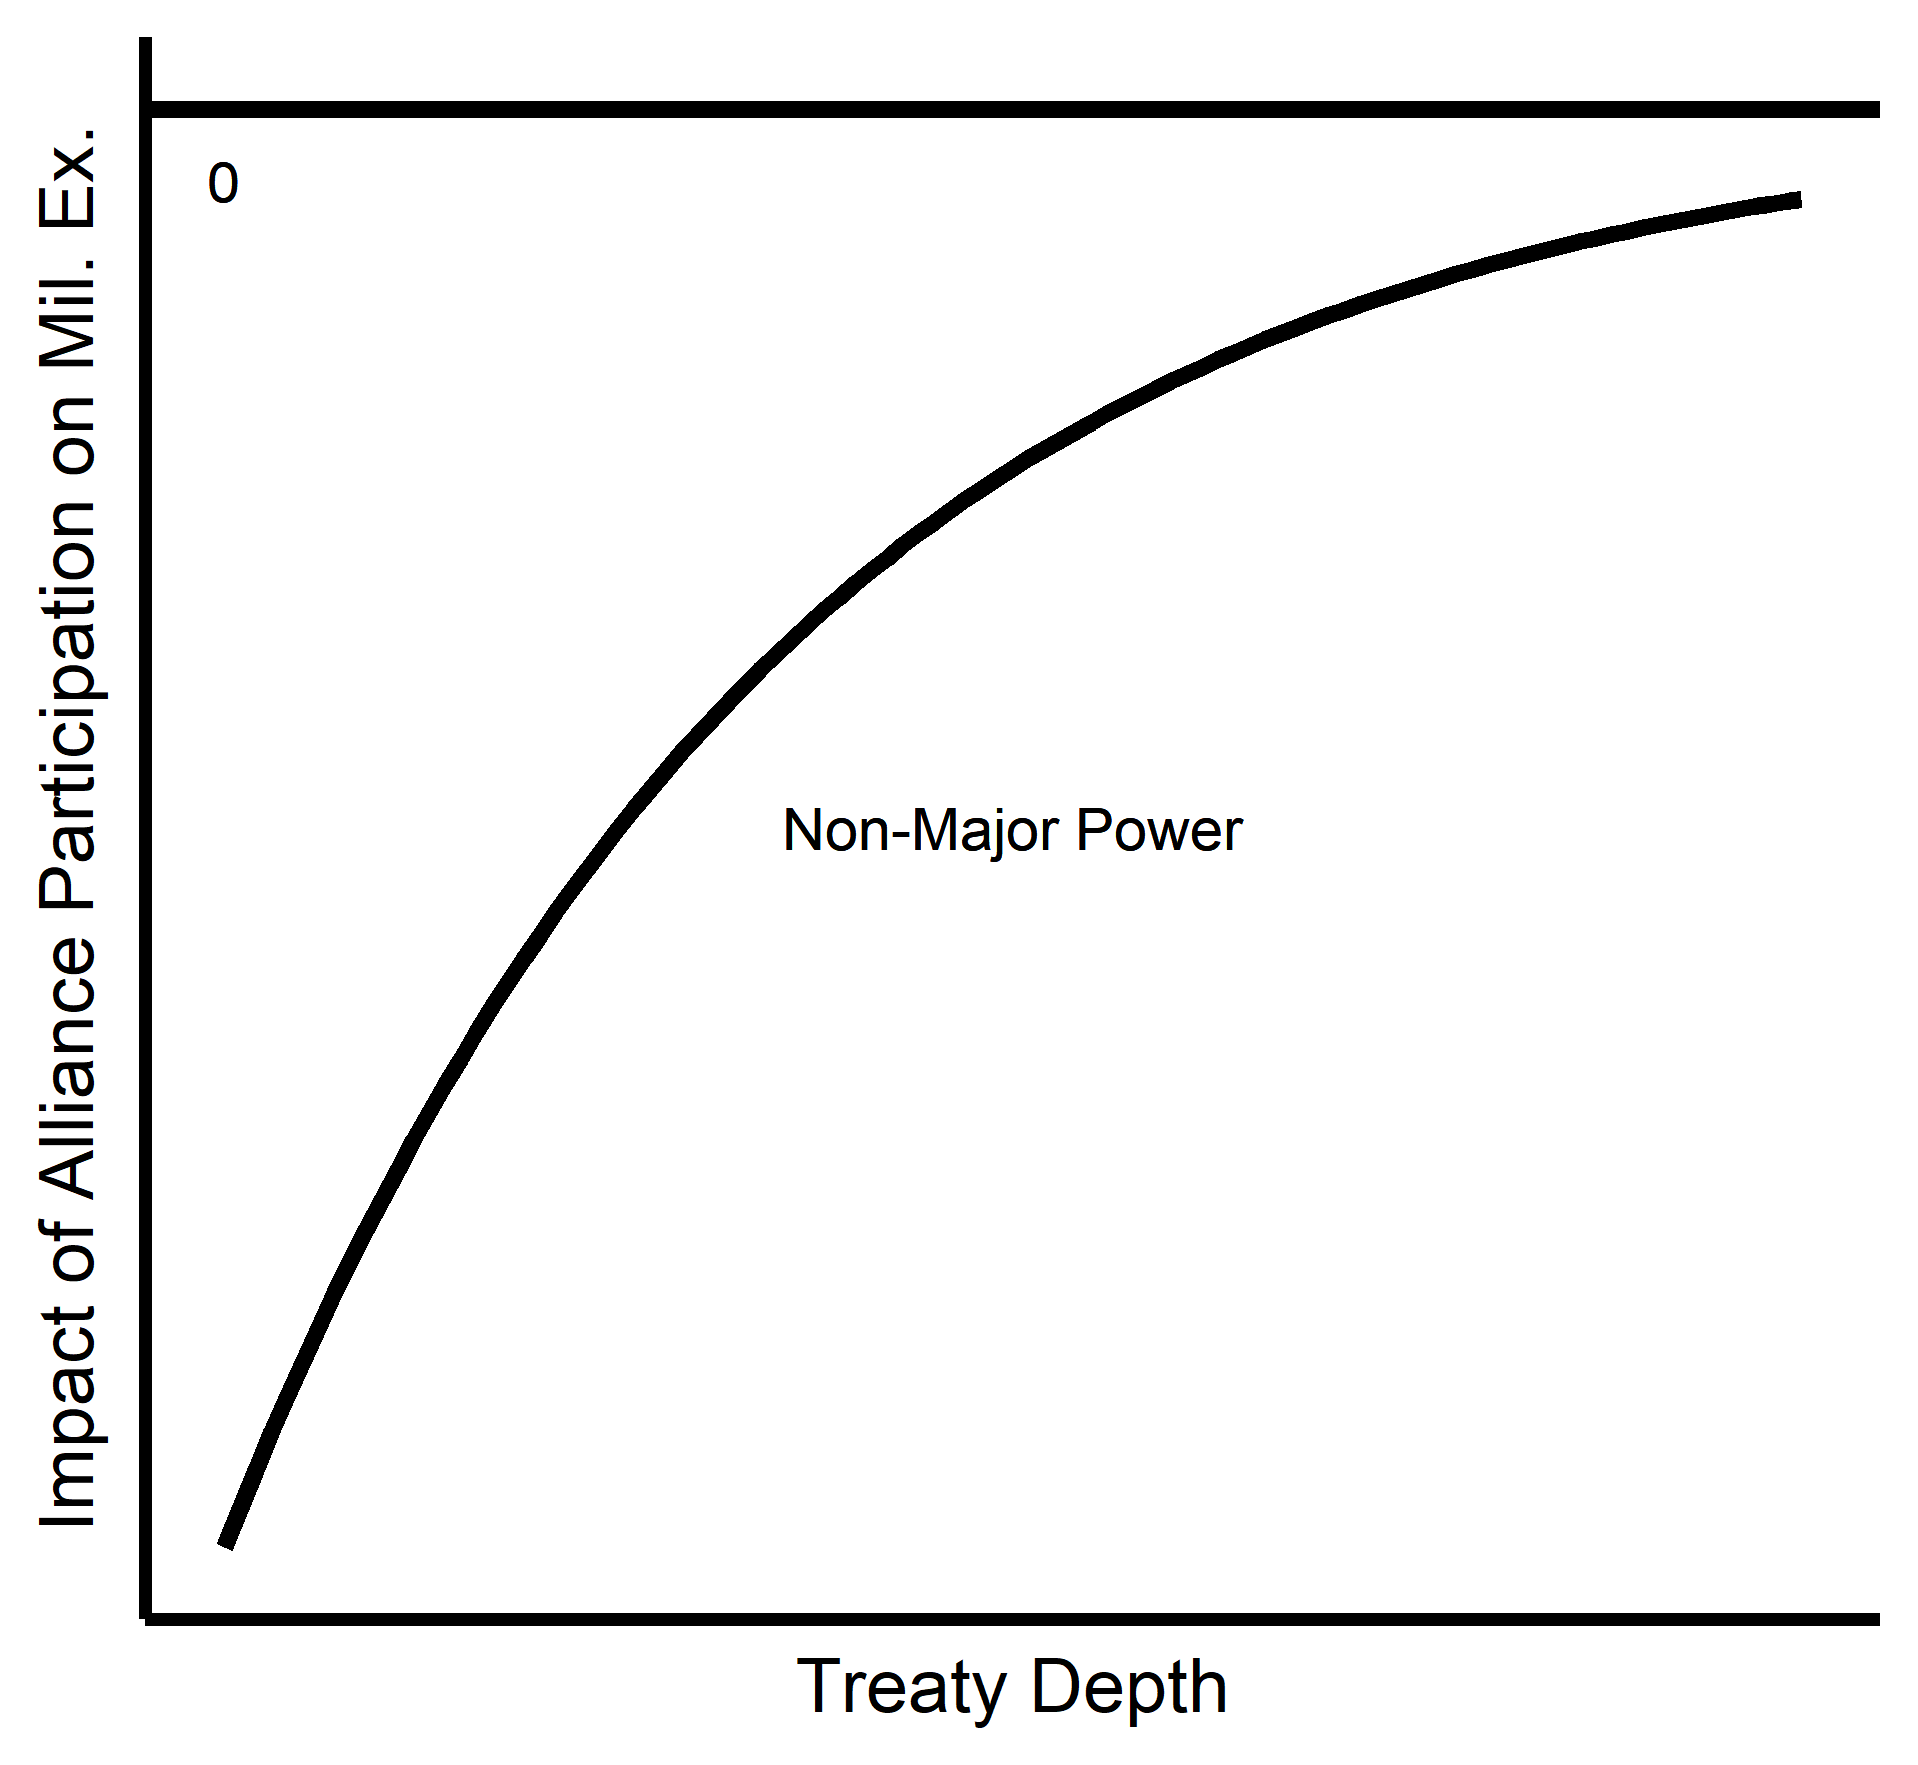
\includegraphics[width=0.95\textwidth]{../figures/illus-arg.png}
	\caption{Abstract illustration of the link between treaty scope and the impact of alliance participation on military spending.
	The top curve represents changes in the impact of alliance participation on growth in major power military spending as treaty scope increases.
	The bottom curve plots the same function for non-major powers.}
	\label{fig:illus-arg}
\end{figure}


\autoref{fig:illus-arg} illustrates my claims about military spending by plotting a hypothetical link between treaty scope and the impact of alliance participation on military spending. 
The top curve shows a possible relationship for major powers, while the bottom curve tracks the same association for non-major powers. 
I do not derive a formal function connecting scope and the impact of alliance participation, so the symmetry, shape and levels of the curves are not essential to the argument.
Instead, \autoref{fig:illus-arg} shows the need to be careful moving between changes in spending growth and changes in levels. 


For major powers, lower military expenditure growth as treaty scope increases could still produce higher spending levels. 
Greater treaty scope reduces the positive correlation between treaty participation and military spending among major powers. 
Even a broad treaty may increase growth in military spending, so lower growth in spending need not reduce the level of major power military spending. 


For non-major powers, increasing growth in spending from expanding treaty scope may still reduce expenditure levels. 
Broad treaties attenuate the negative correlation between alliance participation and military spending in non-major powers. 
But so long as growth remains negative, the level of military spending will fall. 


% Transition para
Because my argument focuses on differences between broad and narrow treaties, the research design must compare treaties and measure alliance treaty scope.  
I use a measurement model to infer treaty scope from formal content, then connect alliances to state military spending with a multilevel model. 
The next section describes the research design in more detail. 



\section{Research Design} 


% two contributions: Develop latent str. measure and then put it into an ML model
The research design makes two contributions. 
First, I develop a latent measure of alliance treaty scope. 
Second, I employ that measure in a multilevel model, connecting alliance-level variation with state-level outcomes. 
To examine differences between major and non-major powers, I estimate the multilevel model in separate samples of major and non-major powers from 1816 to 2007. 
The next section describes the measure of alliance treaty scope. 


\subsection{Measuring Alliance Treaty Scope} 


% Intuituion behind latent measures: observed char reflects underlying concept
My argument implies observed alliance promises reflect the underlying scope of the treaty. 
Broad treaties contain more costly promises. 
Therefore, I use observed alliance characteristics to infer treaty scope.


Treaty scope depends on the potential costs of military support and supplementary sunk cost promises in the pact. 
Potential costs are tied to core commitments of defensive or offensive military support, and conditions on support.\footnote{Some alliances promise only neutrality, consultation, or non-aggression, rather than military support.}  
Sunk costs promises in alliances include integrated military command, forming international organizations, basing rights, promises to make other agreements, and economic or military aid. 


Using observed treaty conditions as indicators of underlying scope could produce two measures. 
One possible measure is an additive index of treaty scope, where treaties with multiple costly promises have higher index values. 
This assumes each indicator is equally important, which is unlikely. 
Instead, I employ latent variable modeling, which is a more flexible way to use observable characteristics to infer an underlying trait. 


Latent variable modeling is a flexible and intuitive way to measure alliance treaty scope. 
My argument expects that there is a single factor underlying variation in potential and sunk costs across treaties.  
The measurement model estimates the correlations between alliance treaty content and the underlying formal scope to predict the scope of each treaty. 


% Justify use
Measurement models have a rich history in political science and have produced notable measures of ideology \citep{Clintonetal2004}, democracy \citep{TreierJackman2008} and human rights \citep{Fariss2014}. 
\citet{BensonClinton2016} use the mixed factor analysis model of \citet{Quinn2004} to measure alliance scope, depth and capability.
I emulate Benson and Clinton's approach, but employ more indicators of scope and a better estimator. 


% How the model works
I use the Bayesian Gaussian Copula Factor Model of \citet{Murrayetal2013} to measure alliance treaty scope. 
Murray et al's model improves mixed factor analysis for continuous, ordinal, and binary observed data by relaxing distributional assumptions. 
Given discrete observed variables and non-Gaussian latent variables, the dependence among the latent variables and their marginal distributions are both influenced by the latent variables.
This model encodes the dependence structure of multivariate latent data using a copula\footnote{Copulas are distribution function on $[0, 1]^p$ where each univariate marginal distribution is uniform on $[0,1]$. This function encodes the dependence structure of a multivariate distribution.} and expresses the latent variables and factor loadings as a series of latent normal variables. 
The semiparametric approach breaks the dependence between the latent factors and marginal distributions, improving inferences about the latent variable. 


Besides the semiparametric component, this measurement model employs a general factor analytic approach.
Factor analysis estimates the association between observed variables and some latent factor.
Each observed variable has a factor loading--- the association between the observed variable and the latent variable.  
Like standardized regression coefficients, factor loadings range from -1 to 1, so observed variables are positively or negatively correlated with the latent factor.  


For each observation, a linear combination of observed alliance characteristics predicts latent treaty scope, like a regression with an unobserved outcome.  
I estimated the model using observed data from all 745 alliances in the alliance-level ATOP data \citep{Leedsetal2002}. 
Indicators of treaty scope are divided between the potential costs of abrogation and sunk costs commitments.
The potential costs depend on promises of defensive support, offensive support, neutrality, consultation, non-aggression and unconditional military support. 
Sunk costs include military aid, economic aid, bases, international organization formation, integrated military command, as well as promises to form new agreements in multiple issue areas and to forgo competing alliances. 
The argument suggests there is a single latent factor underlying variation in all 13 indicators, so I fit the model with one latent factor. 


I used Parameter expanded Gibbs sampling, the default generalized double Pareto (GDP) prior, 10,000 burn-in iterations of the MCMC chain, and 20,000 samples thinned every 20 observations to ensure convergence. 
The estimates include posterior distributions for the factor loadings and the latent factor. 
Because treaty scope is the quantity of interest, I focus on the posteriors of the latent factor. 


% Show the measure for all alliances- note I'll only focus on treaties w/ military support.
Each alliance has a unique posterior distribution of its latent scope. 
I use the mean of that posterior to measure treaty scope. 
\autoref{fig:ls-summary} describes the latent measure for ATOP alliances  with military support from 1815 to 2016.
I examine the 289 treaties offering military support because prior studies of alliance participation and military spending emphasize these treaties.\footnote{
I estimated the measurement model on all alliances to capture the contributions of defensive and offensive conditions to treaty scope.}
Each alliance has a unique scope, so the measure captures the expected scope of an alliance treaty, conditional on the formal promises it makes. 


There is substantial variation in the scope of alliance treaties. 
The top panel of \autoref{fig:ls-summary} is a histogram of mean treaty scope for alliances promising military support. 
Variation between these treaties is driven by sunk costs promises and conditions on military support. 
Most treaties are concentrated between .5 and 1.5 on the latent scale, but approximately 40 treaties fall outside this range. 
The bottom panel of \autoref{fig:ls-summary} plots the posterior means and uncertainty in those estimates against the start year of the treaty. 
Even after accounting for posterior uncertainty, it is possible to distinguish between treaty commitments. 


\begin{figure}
	\centering
		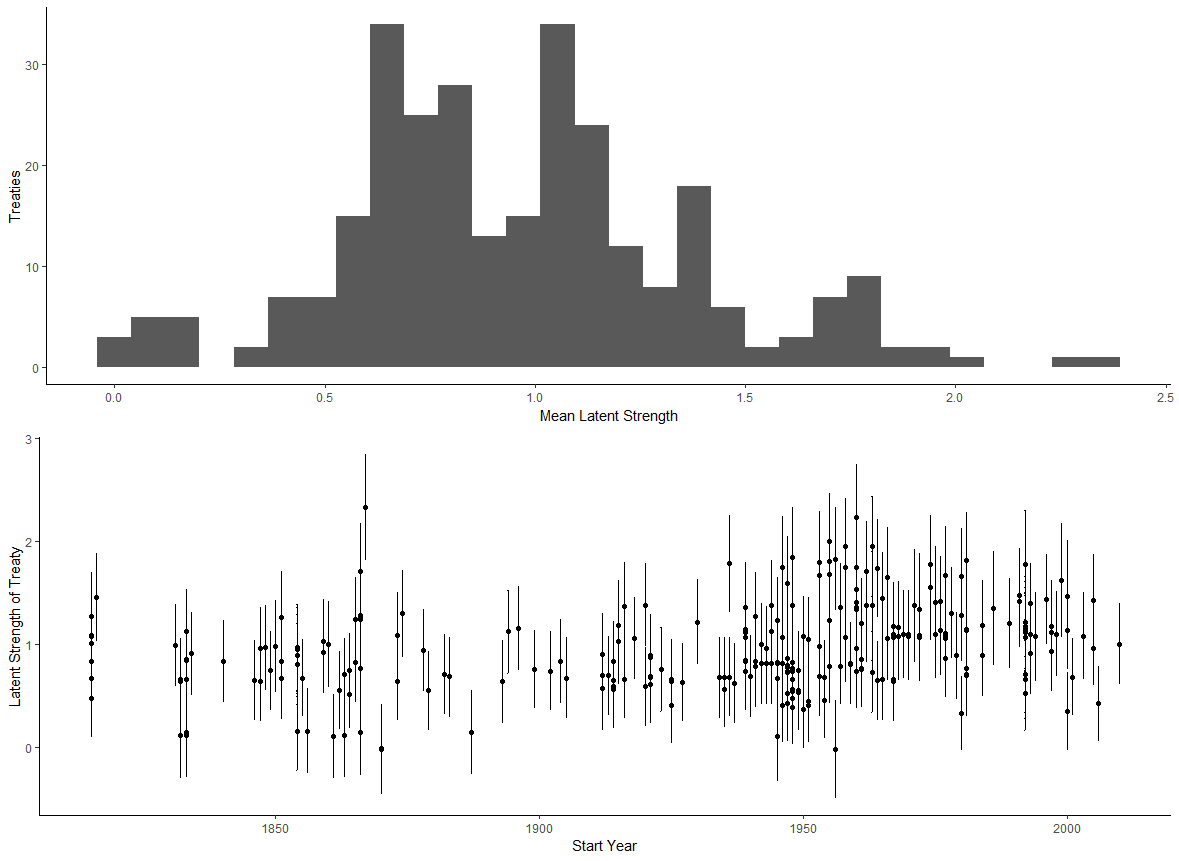
\includegraphics[width=0.95\textwidth]{../figures/ls-summary.png}
	\caption{Summary of latent measure of alliance treaty scope for 289 alliances promising military support from 1816 to 2016. The top panel is a histogram of the expected of alliance treaty scope. The bottom panel plots mean treaty scope (points) and the standard deviation (error bars) against the start year of the treaty.}
	\label{fig:ls-summary}
\end{figure}


% Cases- especially broad and narrow treaties
Although the values of the latent measure are not intrinsically informative, differences between treaties on the latent scale are meaningful. 
The mean of treaty scope is 0.92, and the median is 0.90. 
The median treaty is an 1854 agreement between Austria, France, and Britain against Russia in the Crimean war (ATOP ID 1180). 
The most limited treaty is an 1870 neutrality and offense pact between France and Britain (ATOPID 1300), which Britain used to protect Belgian neutrality during the Franco-Prussian war.  
Britain formed an identical alliance with Prussia in 1870, which scores nearly the same on the latent measure.\footnote{
Sampling variation means the scores will not be exactly the same.} 
Both treaties have only offensive and neutrality promises, conditional on France and Prussia respecting Belgian neutrality, so these two alliances are quite narrow. 


NATO (ATOPID 3180) has a mean latent scope of 0.73, placing it in the second quartile of military alliances. 
NATO's two costly provisions are the defense obligations in Article 5 and establishing the Atlantic Council. 
According to the ATOP coding sheet for NATO, ``There are numerous bilateral agreements among NATO members re: military aid, bases, etc. but they do not qualify as separate alliances, nor are they part of the overall NATO structure.''
The NATO treaty is below average in formal scope in part because additional commitments fall outside the formal treaty.    


The three broadest treaties are an 1867 alliance between Prussia and Hesse (ATOPID 1290), a 1955 treaty between Greece, Turkey and Cyprus (ATOPID 3400) and the United Arab Republic (ATOPID 3300).  
All these treaties supplement promises of military support with other costly cooperation. 
The Prussia--Hessian treaty formed on the eve of war with Austria and includes military aid, integrated military command and basing agreements in addition to offensive and defensive promises. 
The United Arab Republic attempted to unify Syria and Egypt, so it commits to defense, integrated command, military aid, multiple international organizations, and basing rights. 
In the alliance between Greece, Turkey, and Cyprus, Greece and Turkey set up military aid, an integrated military command and international organizations to mange relations on the island.
These extra commitments made arrangements between historic enemies in Cyprus more credible. 
The UAR and Greco-Turkish treaties were undone by domestic coups in Turkey and Syria, but that does not diminish the breadth of cooperation they sought. 


The latent measure has some face, concept, and discriminant validity. 
For face validity, the UAR is a broader commitment than a promise to respect Belgian neutrality. 
The most narrow treaties make few costly promises beyond military support, matching my conceptualization of treaty scope. 
Last, this measure can distinguish between broad and narrow commitments. 


My argument uses variation in treaty scope between alliances to explain growth in military spending.
Broad and narrow treaties should have different effects. 
Differences in scope at the alliance level modifies the impact of alliance participation on growth in military spending at the state-year level. 
Therefore I use a multilevel model to estimate the association between treaty scope and alliance members' military spending.  
The next section summarizes the multilevel model. 


\subsection{Multilevel Model} 


% Best fit for theoretical process. Can compare alliances. 
Multilevel modeling is a natural way to bridge levels of analysis.
This model estimates heterogeneous effects of alliance participation on military spending and uses treaty characteristics to explain variation across alliances. 
I can simultaneously make inferences about the specific impact of individual treaties and the general role of treaty characteristics like scope. 
To facilitate computation and interpretation, I fit the model using Bayesian estimation in STAN \citep{Carpenteretal2016}.\footnote{See the appendix for details of the weakly informative prior distributions and evidence the chains converged.}


This research design adds complexity to a traditional panel data model. 
But the additional components generate novel inferences that connect the argument and research design. 
My predictions emphasize differences in treaty scope, so an alliance level regression in the model contains a corresponding coefficient.
Relying on a state-level proxy for alliance strength compares states rather than alliances and reduces variation in the key independent variable.


Aggregating variables at a different level of analysis may produce misleading inferences \citep{McElreath2016}. 
Multilevel modeling retains the structure of the data, where states are members of multiple alliances. 
Connecting the alliance and state level of analysis then allows me to infer how alliance-level variation impacts annual growth in state military expenditures. 


Besides connecting alliance and state level variation, the multilevel model generates novel comparisons between alliances by estimating the specific impact of each alliance on members' military expenditures. 
Partial pooling of these alliance-specific parameters generates reasonable estimates for every treaty, which can then be used to compare treaties. 
The next section details the model specification. 
 


\subsubsection{Model Specification} 

% Two separate but connected regressions
% State-level regression- alliances enter through spending matrix.
This multilevel model connects two distinct regressions. 
The base is a state-year-level regression, which is similar to a random effects panel data regression.
Then an alliance-level regression modifies parameters in the state-level regression, like an interaction. 


The state-level regression starts with a distribution for the outcome:
\begin{equation}
y \sim student_t(\nu, \mu, \sigma)
\end{equation}
 

$y$ is the dependent variable--- growth in military spending. 
I model spending growth using a t-distribution with degrees of freedom $\nu$ to address heavy tails.\footnote{I estimate $\nu$ directly.}
$\sigma$ is analogous to the error term in a frequentist regression--- this captures unexplained variation in spending growth.  
$\mu$, the mean of the outcome, depends on several covariates.
\begin{equation}
\mu = \alpha + \alpha^{st} + \alpha^{yr} +\textbf{W}_{n \times k} \gamma_{k \times 1}  + \textbf{Z}_{n \times a} \lambda_{a \times 1} 
\end{equation}


Growth in spending is a function of an overall intercept $\alpha$, state and year varying intercepts $\alpha^{st}$ and $\alpha^{yr}$ and a matrix of state-level control variables $\textbf{W}$.
These components comprise a standard random effects model. 
The $\textbf{Z} \lambda$ term incorporates alliance participation.


$\textbf{Z}$ is a matrix of state participation in alliances. 
Columns correspond to each of the $a$ alliances in the data, and rows to state-year observations. 
If a state is not part of an alliance, the corresponding cell of the matrix is zero.
If a state is part of an alliance in a given year, the matrix element contains the log of total allied military spending.


I use total allied spending in the alliance participation matrix because more capable alliances provide extra benefits.
Increasing allied capability makes promises of military support more valuable \citep{Johnsonetal2015}.  
$\textbf{Z}$ encodes a quasi-spatial indicator of alliance participation for all $a$ alliances in the data. 
States can be members of multiple treaties at once, so observations are not neatly nested. 
This specification allows each alliance to have a unique impact on military spending, even when states participate in multiple treaties. 


$\lambda$ is a vector of parameters which estimate the impact of participation in specific alliances on military spending. 
Because the non-zero elements of $Z$ are allied spending, the $\lambda$ parameters capture alliance members' responsiveness to greater allied capability. 
Each alliance has a unique $\lambda$, which comes from a common distribution. 
The shared distribution assumes alliances are similar but different in how they impact growth in military spending. 


% Alliance-level regression:
The second part of the multilevel model uses alliance characteristics to predict how alliance participation is associated with growth in military spending. 
The $\lambda$ parameters are the outcome in an alliance-level regression.
Therefore the impact of alliance participation on members' military spending depends on treaty characteristics, including scope. 
In this second-level regression: 

\begin{equation}
\lambda_{a} \sim N(\theta_{a}, \sigma_{all})
\end{equation} 
and 
\begin{equation}
\theta_{a} = \alpha_{all} + \beta_1 \mbox{treaty scope} + \textbf{X}_{a \times l} \beta
\end{equation}


% Like an interaction between alliance and state-level factors 
In the alliance-level regression, $\textbf{X}$ is a matrix of the $l$ alliance-level control variables and $\alpha_{all}$ is the constant.
Adding $\sigma_{all}$ means predictions of $\lambda$ are not deterministic--- the alliance level regression contains an error term. 
Increases in $\sigma_{all}$ imply greater variation in how alliance participation impacts military spending. 
The second-level regression includes treaty scope, and each $\beta$ parameter modifies the impact of alliance participation on growth in military spending. 
The $\beta$s are like marginal effects in an interaction. 


Treaty scope impacts military spending by changing the consequences of alliance participation.
This is an indirect link, but it matches my argument that scope modifies the impact of alliance participation on military spending.  
Changing treaty scope shifts $\lambda$, which in turn affects growth in military spending.
Hypothesis 1 predicts $\beta_1$ will be negative among major powers, and Hypothesis 2 expects $\beta_1$ will be positive for non-major powers.
$\beta_1$ compares broad and narrow treaties in each sample. 


% Provide an example observation
Consider one observation as an example of how the model works. 
Growth in Argentina's military spending in 1955 depends on Argentina's economic growth, political regime, conflict participation, and rival military spending. 
Argentine participation in the Rio Pact and OAS also changes growth in spending through allied capability. 


\begin{equation}
\begin{split}
& \mbox{Argentina 1955} = \mbox{Overall mean}
+ \mbox{Argentine Intercept} + \mbox{1955 Intercept} 
+ \mbox{Argentine Characteristics} \\
& + \lambda_{OAS} * \mbox{OAS Expenditure} + \lambda_{Rio} * \mbox{Rio Pact Expenditure}
\end{split} 
\end{equation}


$\lambda_{OAS}$ and $\lambda_{Rio}$ capture the impact of participating in each alliance and are a function of the alliance level regression. 
Key characteristics of the OAS and Rio pact alter their respective $\lambda$ parameters.
Other alliances have no impact on growth in Argentine military spending. 


In this model, the $\beta$ parameters capture the general association between key alliance characteristics and military spending. 
The $\lambda$ parameters express the impact of participation in each alliance, permitting heterogeneous effects of different treaties. 
Using alliance characteristics to modify the impact of alliance participation matches my conditional argument. 
I now describe the sample and covariates in the analysis.  



\subsection{Sample and Covariates} 

% Sample of states 
I estimate this model on two samples of states from 1816 to 2007--- one sample of major powers, the other of non-major powers. 
Splitting the sample means I cannot directly compare estimates from the major and non-major power samples, but it shows different trends in the two samples. 
A split sample followed by graphical comparison of the estimates is a simple approximation of letting the slopes vary \citep{GelmanHill2007}. 
If major powers focus on influence and non-major powers emphasize immediate territorial security, the data generating processes for military spending in major and non-major powers are likely different.
Therefore alliance-level coefficients besides strength will vary between major and minor powers and splitting the sample is a simple way to capture these distinctions.\footnote{I also estimated a varying slopes model, which generates similar inferences about treaty scope. More information on that model and the results is available in the appendix.} 
Alliance participation data comes from the ATOP project \citep{Leedsetal2002}. 
I focus on participation in defensive and offensive treaties, because prior studies of alliances and military spending examine these treaties. 


% sample of alliances: restricted to treaties with military support
I classify state-year observations in each sample using a measure of major power status from the Correlates of War Project. 
As with the argument, this is a course division. 
Even so, it matches the sharp comparison in the argument and employs a widely used measure. 


The non-major power sample contains 8,668 observations in the state-level regression, and 192 alliances. 
There are 930 major power observations and 148 alliances. 
Although the major power sample is smaller and has fewer states, Bayesian estimation should generate plausible estimates \citep{Stegmueller2013}. 


% DV: growth in milex
The state-year dependent variable is growth in military spending.
Growth in military expenditures is calculated as:
\begin{equation}
\mbox{Growth Mil. Expend} = \frac{ \mbox{Change Mil. Expend}_t }{ \mbox{Mil. Expend}_{t-1} }
\end{equation} 
I used the Correlates of War Project's data on military spending to measure spending growth \citep{SingerCINC1988}. 
Growth in spending is equal to changes in spending as a share of the previous year's military spending, so changes are relative to previous levels of spending. 


Using military expenditure growth as the dependent variable has several benefits for the research design. 
The level of military spending is not stationary for most states, especially in longer panels. 
Thus, using growth in spending in regression models limits the risk of spurious inferences.
Benchmarking changes to prior expenditures also facilitates comparisons across states and over time. 


% key IV: mean treaty scope
The key independent variable is the mean latent scope of each alliance. 
This variable enters the model in the alliance-level regression. 
I also include a series of state and alliance-level controls. 


% Describe covariates at each level. 
In the state-level regression, I adjust for several variables that are correlated with alliance participation and military spending. 
State-level covariates include GDP growth \citep{Boltetal2018}, regime type, international war \citep{Reiteretal2016}, civil war participation \citep{SarkeesWayman2010}, annual MIDs \citep{Gibleretal2016}, rival military spending \citep{ThompsonDreyer2012} and a dummy for Cold War years.
Conflict participation, alliances, and military spending are all correlated \citep{SeneseVasquez2008}. 
I include growth in GDP instead of levels of GDP because GDP levels are non-stationary, and economic growth shapes the opportunity costs of military spending \citep{Kimball2010, Zielinskietal2017}.


The alliance-level regression contains the mean of the latent treaty scope--- the key independent variable. 
Other alliance level variables are correlates of treaty design and military spending, including the number of members and share of democracies in a treaty at time of formation \citep{Chibaetal2015}.
I adjust for superpower membership--- whether the US or USSR participated in a treaty during the Cold War. 
Two dummy indicators of wartime alliances and asymmetric obligations \citep{Leedsetal2002} complete the alliance-level regression specification. 
Wartime alliances often require higher spending and broad commitments, while asymmetric obligations may add to spending by major powers while reducing non-major power spending. 


Adjusting for all of these covariates helps address systemic differences between states and alliances from strategic selection into alliances. 
Regime type and external threat are especially important in that endeavor. 
The next section describes the results from the major and non-major samples.
 

\section{Results}


Results are based on 2,000 total samples from four chains, with 1,000 warm-up iterations. 
To facilitate model fitting, I employed a non-centered parameterization of the varying intercepts and a sparse matrix representation of \textbf{Z}. 
Standard convergence diagnostics indicate the chains adequately explored the posterior density.\footnote{See the appendix for more details on convergence.} 


% note on interpreting Bayesian results
Because I use Bayesian modeling to estimate the association between treaty scope and growth in military spending, each coefficient has a posterior distribution--- the likely values of the coefficient conditional on the priors and observed data.
There are no indicators of statistical significance. 
Instead I calculate the negative and positive posterior probability for the two treaty scope coefficients to assess Hypotheses 1 and 2.


% show latent strength coefficient in each subset of data
\begin{figure}[htbp]
	\centering
		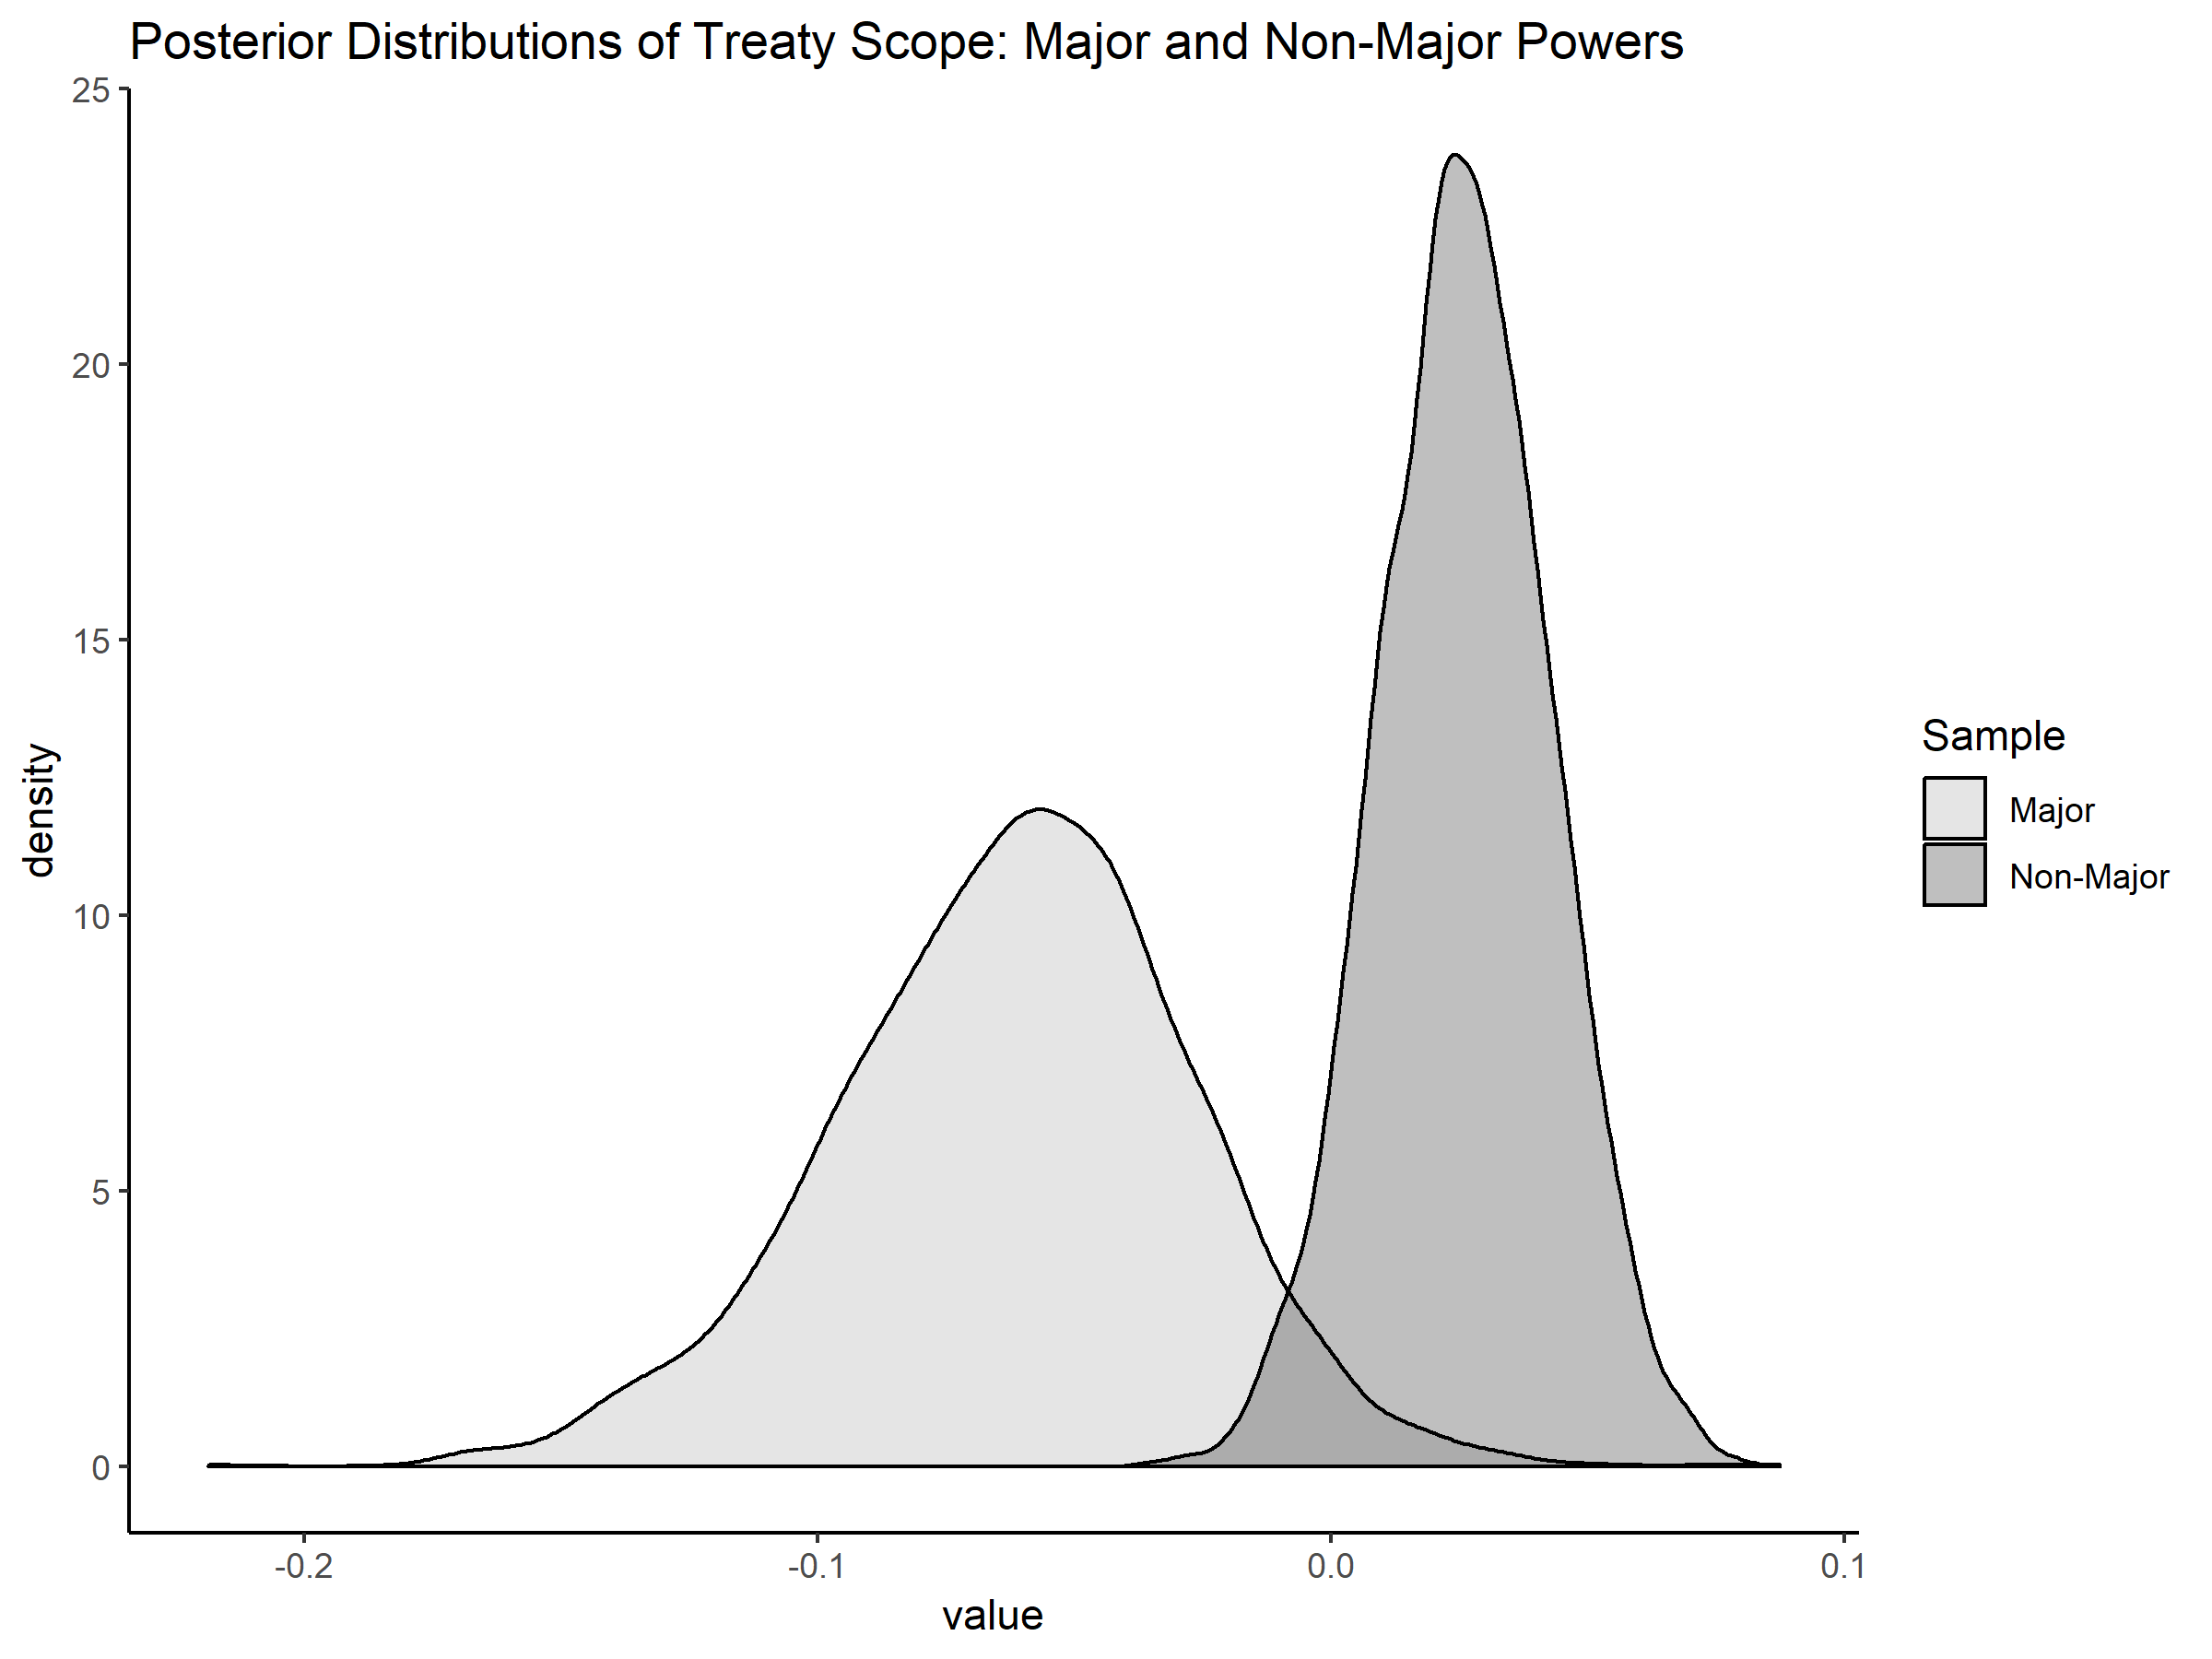
\includegraphics[width=0.95\textwidth]{../figures/scope-dens-split.png}
	\caption{Posterior density of treaty scope coefficient in major and non-major power samples, 1816 to 2007. 96\% of the major power posterior mass is negative. 94\% of the non-major power posterior mass is positive.}
	\label{fig:str-dens}
\end{figure}


\autoref{fig:str-dens} plots the full posterior density of the treaty scope coefficients in the major and minor power samples.\footnote{The smaller major power sample increases variance in all the coefficient estimates.} 
96\% of the posterior mass for major powers is negative. 
94\% of the posterior mass for minor powers is positive. 


The preponderance of evidence matches the predictions of Hypotheses 1 and 2. 
For major powers, there is a 96\% chance increasing treaty scope is associated with lower growth in military spending. 
There is a 94\% chance greater treaty scope is associated with higher growth in military spending for non-major powers.


Though the two coefficients have the expected sign, more evidence is needed to establish substantive importance. 
To assess the substantive impact of a change in treaty scope, I compare the expected value of the coefficient to typical growth in military spending in each sample. 
Among major powers, the mean of the treaty scope coefficient is -0.05, and median growth in military expenditures is 0.04.\footnote{The median is a better summary of the dependent variable because large positive and negative outliers influence the mean.} 
So a one-unit increase in treaty scope more than offsets the typical annual growth in military spending. 
This change in spending is a plausible effect--- 5.1\% of the 2018 US defense budget was spent directly on NATO.\footnote{See this \href{https://www.iiss.org/blogs/military-balance/2018/07/us-and-nato-allies-costs-and-value}{blog post from the IISS}.} 


For non-major powers, the mean of the treaty scope coefficient is 0.03, and median growth in military expenditures is 0.06. 
Greater treaty scope increases growth in minor power military expenditures by about half of typical growth. 
In both the major and non-major power samples, the expected impact of higher treaty scope has a large substantive effect.\footnote{Of course, uncertainty in the posterior estimates includes larger and smaller effects.}


I also assess substantive importance by looking at patterns in the $\lambda$ parameters. 
Each $\lambda$ measures the impact of treaty participation. 
If treaty scope has a large influence on alliance participation, it will appear in the $\lambda$ estimates. 
There should be a negative trend in the expected value of $\lambda$ as treaty scope increases in major power alliances and a positive trend among non-major power alliances. 


\begin{figure}[htbp]
	\centering
		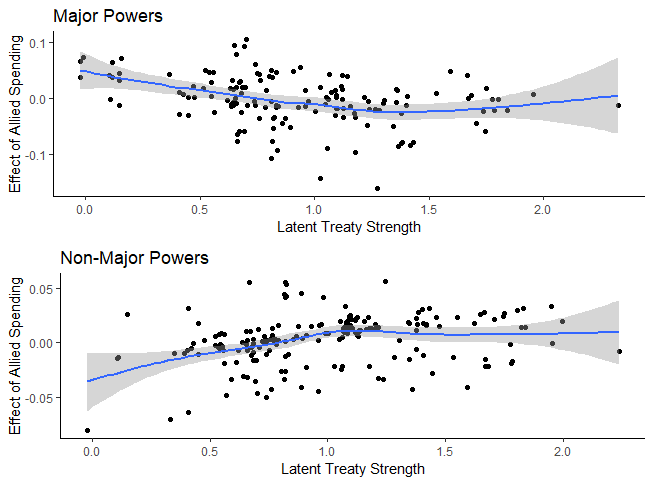
\includegraphics[width=0.95\textwidth]{../figures/lambda-ls-scatter.png}
	\caption{Scatter plots of trends in mean $\lambda$ parameters and treaty scope. $\lambda$ is the total impact of alliance participation on growth in military spending. The top panel is major powers, where this is a negative trend between $\lambda$ and treaty scope. In the bottom panel the same trend is positive for non-major powers. Trend lines estimated using linear regression.}
	\label{fig:lambda-ls-scatter}
\end{figure}


\autoref{fig:lambda-ls-scatter} plots the expected value of $\lambda$ across the range of treaty scope in the two samples. 
In the major power sample, there is a negative trend in the scatter plot.
For non-major powers, the trend is positive.
The correlation between mean $\lambda$ and treaty scope is statistically significant in both samples. 


These trends match the underlying logic of Hypotheses 1 and 2. 
Limited treaties tend to increase growth in defense spending for major powers, but that positive association falls as treaty scope increases. 
Narrow treaties often reduce growth in military spending among non-major powers, while most broad treaties have a less negative effect. 
Because other treaty characteristics and unmeasured factors also influence the $\lambda$ estimates, not all treaties conform to the expectations of decreasing or increasing growth in spending. 


Trends in the $\lambda$ parameters across the range of treaty scope suggest that treaty scope has a substantial impact. 
Even after accounting for other alliance characteristics, alliance strength drives the impact of alliance participation down for major powers, and up for non-major powers. 
Alliance treaty scope is a key source of heterogeneity in how alliance participation impacts military spending. 


While the statistical model estimates general associations, it does not show the underlying process. 
To further illustrate the explanatory power of my argument, the next section offers a brief description of US alliance politics.   
I focus on NATO--- the most important alliance in the international system.  


\section{NATO, Treaty Scope and Military Spending}


% generally limited treaties 
US foreign policy after World War II illustrates the tradeoff between entanglement and influence for major powers.
American choices in treaty design also had important consequences for junior partners. 
While forming alliances, the United States balanced between fear of ``foreign entanglements'' and maintaining influence to check the USSR.
The Soviet threat led US policymakers to form several alliances, but domestic opposition weakened the formal promises in most treaties. 
Most US treaties contain few formal promises besides defense against aggression.  


% NATO 
NATO shows how limited commitments led to additional defense outlays to support Washington's influence.
After the end of World War II, the United States sought to protect Europe from the USSR. 
Despite concern about Soviet intentions, isolationists in the US Senate feared an alliance would force America to intervene automatically if partners were attacked, bypassing the power of Congress to declare war \citep[pg. 280-1]{Acheson1969}.
Therefore Article V states that if one member is attacked the others ``will assist the Party or Parties so attacked by taking forthwith, individually and in concert with the other Parties, \emph{such action as it deems necessary}'' (emphasis mine). 
Military support was and is not guaranteed. 


The absence of automatic US involvement increased demand for reassurance by European allies. 
Europeans feared that if the Soviets invaded, the US would decide not to fight. 
Bilateral agreements on troop deployments then became a means of reassurance. 


In 1950 West Germany formally requested clarification on whether an attack on US forces in Germany would be treated as an armed attack on the United States and US officials said it would \citep[pg. 395]{Acheson1969}. 
A 1951 presentation by Dean Acheson to Dwight Eisenhower argued European allies ``fear the inconstancy of United States purpose in Europe. ... These European fears and apprehensions can only be overcome if we make the necessary full and active contribution in terms of both military forces and economic aid'' \citep[pg. 3]{Acheson1951}.  
But even after agreeing to deploy troops, US policymakers hoped Europeans would soon provide more for their own defense, while acknowledging the United States ``should not dictate what they shall do'' \citep[pg. 2]{Johnson1950}. 


Though the executive branch sought a broad NATO treaty, isolationist fears of foreign entanglement constrained its formal scope. 
Many Senators also opposed military aid to Europe \citep[pg 285]{Acheson1969}, leading to more bilateral bargaining and aid through other channels. 
Due to limited formal sunk costs commitments in the NATO treaty, the US has little leverage on military spending. 
NATO members have been free to reduce growth in defense spending. 


In response, American policymakers from Eisenhower to Trump have attempted to browbeat NATO members into spending more. 
These efforts have usually failed. 
Most European members of NATO have been unresponsive to changes in external threat and US defense spending \citep{PluemperNeumayer2015}. 


The US has threatened to leave NATO in response to this European ``free-riding,'' but those threats were not credible. 
During the Cold War, US interests in containing the USSR trumped irritation with allied free-riding.  
But without other costly treaty commitments to use as leverage, the United States had few ways to check allied incentives to reduce growth in military spending. 


% add something on estimates from ML model
Estimates of the $\lambda$ parameter in the major and non-major power samples corroborate this reading of the NATO case. 
NATO's formal promises are weaker than average among defense treaties. 
In the major power sample, NATO membership adds 0.04 to growth in military spending in expectation.
For non-major powers, NATO membership lowers growth in military expenditure by -0.006 in expectation.\footnote{
The UK and France are major powers from 1945 on, and Germany is a major power after 1991. Therefore, these estimates may underestimate reduced growth in spending by NATO members, because all three of these states relied on US capability for protection. The positive growth in major power spending is driven by the US.}


So the multilevel model estimates match how the argument views NATO.
US fear of entanglement led to a need for growth in military spending and limited bargaining leverage in alliance maintenance. 
European members still gained security, but retained the freedom of action to lower growth in defense spending.   
Evidence from NATO corroborates the expectations and process of my argument. 
This case and the statistical analysis add to our understanding of alliance participation and military spending. 


\section{Discussion}


% Precise interpretation: compares alliances. Not treaty vs absence. 
My findings address the debate over whether alliance participation increases or decreases military spending. 
Claims alliance participation only increases or decreases military spending are inaccurate. 
Major and non-major powers respond differently to alliance participation because they use treaties for different purposes. 
Thus, alliance treaty design has distinct ramifications for major and non-major powers. 
Treaty scope decreases growth in major power spending from alliance participation, while increasing non-major power expenditure growth. 


% Link for force multiplier and foreign entanglement
My argument builds on other conditional arguments about alliance participation and military spending \citep{DigiuseppePoast2016} and clarifies where the force multiplier and foreign entanglement perspectives best apply. 
The force multiplier perspective covers non-major powers well. 
But non-major powers cannot reduce growth in military spending in all alliances, because broad treaties constrain their freedom of action.
The foreign entanglement prediction applies to major powers, but broad treaties provide more influence, lowering the positive correlation between alliance participation and growth in military spending. 


This paper connects previously separate components of the political economy of alliances. 
The first component is work on issue linkage politics in alliances \citep{Mattes2012, Poast2012, Poast2013, Johnson2015}.
The second is the arms-alliances tradeoff \citep{Morrow1993}. 
By using issue linkages to explain when alliance participation increases or decreases military spending, I provide a holistic perspective on the political economy of alliances.  


How do the findings compare to prior evidence on alliance participation and military spending? 
Connecting my findings with earlier evidence requires renewed attention to specific and general research designs. 
General studies compare states in a particular kind of alliances to those without such an alliance. 
Specific studies estimate responsiveness to allied military spending in a few treaties. 


My research design emulates specific studies by estimating the unique impact of participation in individual treaties. 
I then use alliance treaty design to explain variation in how treaty participation impacts growth in military spending.
The key coefficient estimates compare broad and narrow treaties to captures the general consequences of treaty design. 
Therefore, my results encompass specific and general studies. 
I estimate both the impact of individual treaties and general differences between treaties. 


% limitations of RD
This paper has several limitations.
The argument offers a cursory treatment of the domestic political economy of military spending. 
By reducing domestic politics to an assumption that military spending has opportunity costs, which are decreasing in state size, I elide a rich literature on this topic \citep{WhittenWilliams2011, AlptekinLevine2012}. 
Furthermore, domestic politics shapes how states define their foreign policy interests and the tools they use to pursue those interests \citep{Fordham1998, Fordham2011, Narizny2007}.
At the moment, my argument treats foreign policy interests as given.  


My findings also only address formal issue linkages. 
The measure of treaty strength only includes formal promises, in part because informal issue linkages are hard to observe. 
As a result, my test of treaty scope and the associated issue linkages is probably conservative--- it does not capture phenomena my argument expects should have a similar effect. 


% Strategic treaty design
Strategic alliance design is another weakness of the research design. 
Non-random selection into different kinds of alliances could produce systematic differences between members that are not captured for in my statistical model. 
I attempted to control for correlates of alliance treaty scope, but oversights are possible. 


Despite these limitations, the argument and results provide valuable insights about alliance participation and military spending. 
I explain when alliance participation is associated with more or less growth in military spending, addressing debate between the force multiplier and foreign entanglement views of alliances. 
How alliance participation impacts military spending depends on state capability and alliance treaty scope. 
I provide evidence for these predictions using a new measure of alliance treaty scope and a multilevel model. 
The argument and findings have implications for scholars and policymakers. 


\section{Conclusion}

% tie it all together
Alliance participation will not uniformly increase or decrease military spending. 
Both the force multiplier and foreign entanglement views of alliance participation are correct, each in different circumstances.
Alliances are more foreign entanglement for major powers and more force multiplier for non-major powers, but the consequences of alliance participation depend on treaty characteristics.  


% Start conclusion
There are several implications of my findings that treaty scope decreases growth in major power military spending from alliance participation, while increasing growth in spending from alliance participation for non-major powers.  
First, they reinforce the importance of heterogeneity among alliances \citep{Leeds2003, Benson2012, DigiuseppePoast2016}.
Alliances have heterogeneous effects on conflict risk and military spending. 


% Add paragraph on distributional consequences.
Another implication is the distributional consequences of changes in military spending within states and among alliance members.  
Changes in military spending from alliance participation have important distributional consequences. 
By altering growth in military spending, the design of international alliances alters the domestic political economy of member states. 
But the domestic economic consequences of alliance politics are a possible avenue for future research. 


% The argument indicates tradeoff
Besides their scholarly value, the argument and evidence have implications for policy debates. 
The tradeoffs major and non-major powers face in alliance treaty design can guide our understanding of why some treaties lead to ``free-riding'' and policy responses. 
Major powers may be able to check allied free-riding through increasing the scope of their alliance commitments. 
Greater influence can limit allied free-riding, but it requires deeper engagement abroad. 


% Implications for policy. 
The United States is currently wrestling with the implications of treaty scope. 
Washington has often decried ``free-riding'' by allies who provide too little for their own defense \citep{Lanoszka2015}. 
But allies are able to free-ride partly because the US makes limited formal alliance commitments. 
``Foreign entanglements'' may provide more influence to curb falling allied defense spending. 

 
Therefore, growing institutionalization of NATO, including the agreement for all allies to spend at least 2\% of GDP on defense, may increase defense spending.
Increasing obligations within NATO tie the United States more closely to Europe, but are a better check on allied free-riding than verbal exhortations. 
Issue linkage bargaining that connects economic cooperation and defense spending could also lead to higher allied military spending.
Threatening to leave the alliance is not credible and undermines US gains from alliances. 


The United States could use broad formal commitments as a substitute for greater defense effort in reassuring allies.
The danger is that increasing treaty scope could create a situation where obligations exceed capabilities \citep{Kennedy1987}. 
Emboldening junior partners with a broad treaty might have deterrent value \citep{Bensonetal2014}, or increase the risk of conflict \citep{Benson2012}.
Thus, while greater treaty scope can reduce the impact of alliance participation on growth in major power military spending and increase non-major power spending growth, it has other consequences. 
The tradeoffs surrounding alliance treaty scope and how to manage them fall outside this article, but are an important issue for scholars and policymakers to consider. 
Efforts to increase allied military spending may have other consequences, so the policy implications of my findings are complex. 

 



\singlespace
 
\bibliography{../../MasterBibliography} 





\end{document}
